\documentclass{book}
\usepackage{graphicx,makeidx,textcomp,tipa,siunitx,tikz,multicol,hyperref}
\usepackage[utf8]{inputenc}
\usepackage[all]{hypcap}
\renewcommand{\thefootnote}{\fnsymbol{footnote}}
\pdfcompresslevel 9

\title{Eggshell / Plants}
\author{B M Corser}
\date{Janurary -- March 2013}

\begin{document}

\maketitle

\tableofcontents

\chapter{Nature Eruption}

\begin{figure}
\centering
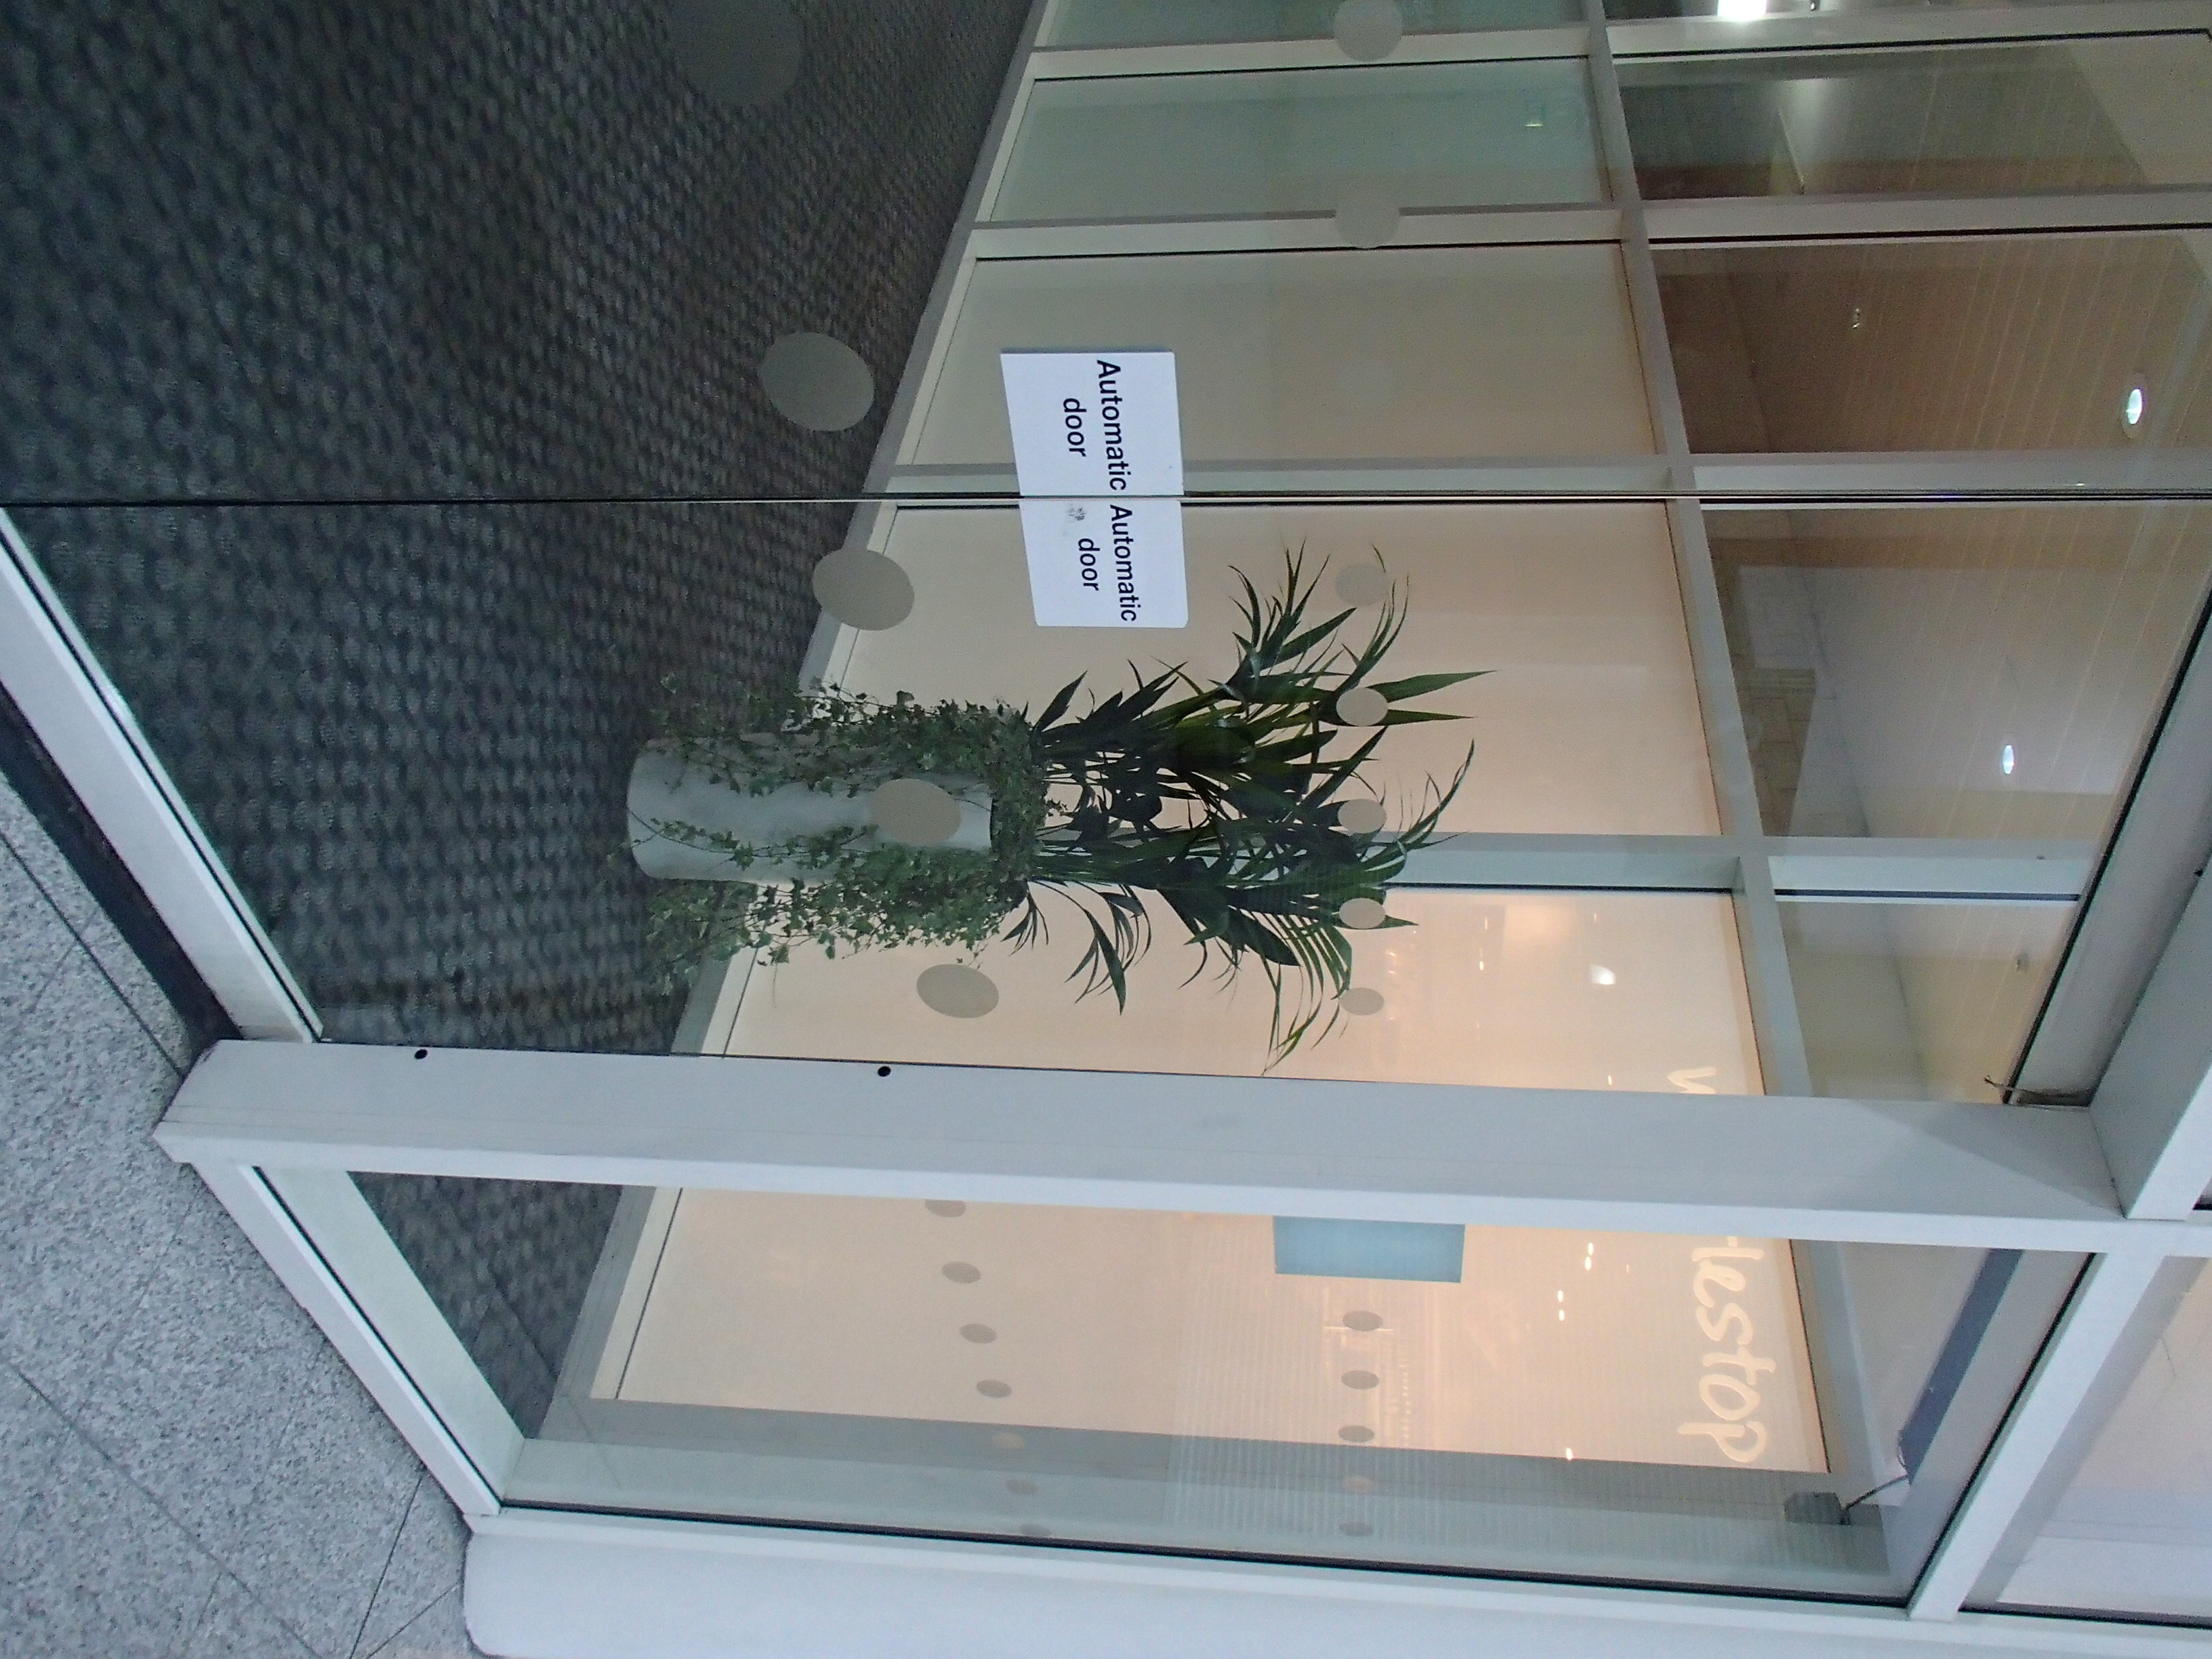
\includegraphics[width=\textwidth,angle=90]{figures/P1050140.JPG}
\caption{Nature Eruption}
\end{figure}

It is only in the quiet of panels, when horror vacui is quietly receded from,
that movement can begin to come from nature. A thing that should not shudder
begins to exhibit the first tremors of life. There is a sensation of bubbling
beneath the feet, a fibrous crunching, something like the tiny sounds at the
bottom of the lungs on a deep breath. There is a kind of panting. Surely an
eruption is coming.

In a regimented frame, there is an attempt to cast authority through the
appearance of order. This is a setting without exclamation. This is not a place
where anything slides luxuriously from upright to reclining, but a desperate
calmness sites itself in the air, an hyperactive stillness. It is not possible
to situate this frame (to give it a context or some kind of Gestalt backdrop),
instead an observer must attempt to impose herself as a figure for the things
she sees to stand a chance of approaching corporeality. This impetus is
well-anticipated in the viewer; a sturdy pastiche of their figure is ``pre''
placed in the scene, already there, waiting to be called into play by this
acknowledgement.

There is no pointed coquettishness or promise, instead there is an air of
hastily concieved urgency, like a dull ambient panic or pale anxiety. The
subtly implied threat of grey and misty Lacanian reality is veiled with extreme
economy of gesture. As lightly as is is possible to contain something is how
things are contained here. It is impressive, then, that this containment is
able to be so utterly complete.

This should surely be the conception of a very sublime perspective, to solve an
issue outside of flesh and to have solved it with so light a touch. It is
difficult to see the weight (or power) that maintains the rigidity holding
things up.  This weight is hidden by design, stacked above head-height, stuffed
inside walls, mirrored away or diguised in large-scale optical illusion.

There is a physical tension around us, it feels like being inside a cat's
cradle. This is not a situation that begs exploration. We explore anyway.

Free movement in this space makes the space itself feel tenuous. It is as if
the whole charade could wink out of existence if a certain or particular floor
tile were stepped on.  \emph{The three of us tread carefully.} We emulate the
stasis through which we find ourselves moving.

Right now, nothing suggests relief will come, the unbroken hush hums lulling
perpetuity and likewise waves of silence ripple and echo from a cavernous
\emph{above}.  The light doesn't obviously come from anywhere, it seems to be
somehow within the beams and panes and floors and walls. The defining edges of
things look drawn on, the definition between things that forms what we can have
as recognisable objects is only made here as an amicable gesture or polite
courtesy. Moreover it is certainly something that we should be grateful for.

But some good change is on its way, the very source of levity itself will soon
spring and be upon us in a shock of lush green. With one glance, the mind
delves into the jungles of the mind, the immediate possibility of an
inhabitance entirely different in character bustles in and brusquely presents
itself. We exclaim \emph{``This is the opposite!''} as creepers and ferns erupt
from below head height, announcing the end of mundane sterility. Beginning at
waist height, spilling voluptuously down to almost touch the floor and
sprouting upwards to reach just below the neckline, fronds elegantly bowing to
the tip.

We find a formality here that appears naturally, without method or intent,
sensual and striking. Flowing arcs effortlessly mixed with staccato points.
Misplaced ribbing and frantic groupings of tiny fluted spouts. And here too
the pure violence and natural struggle that constitute life.

\chapter{Plinth'd Nature}

\begin{figure}
\centering
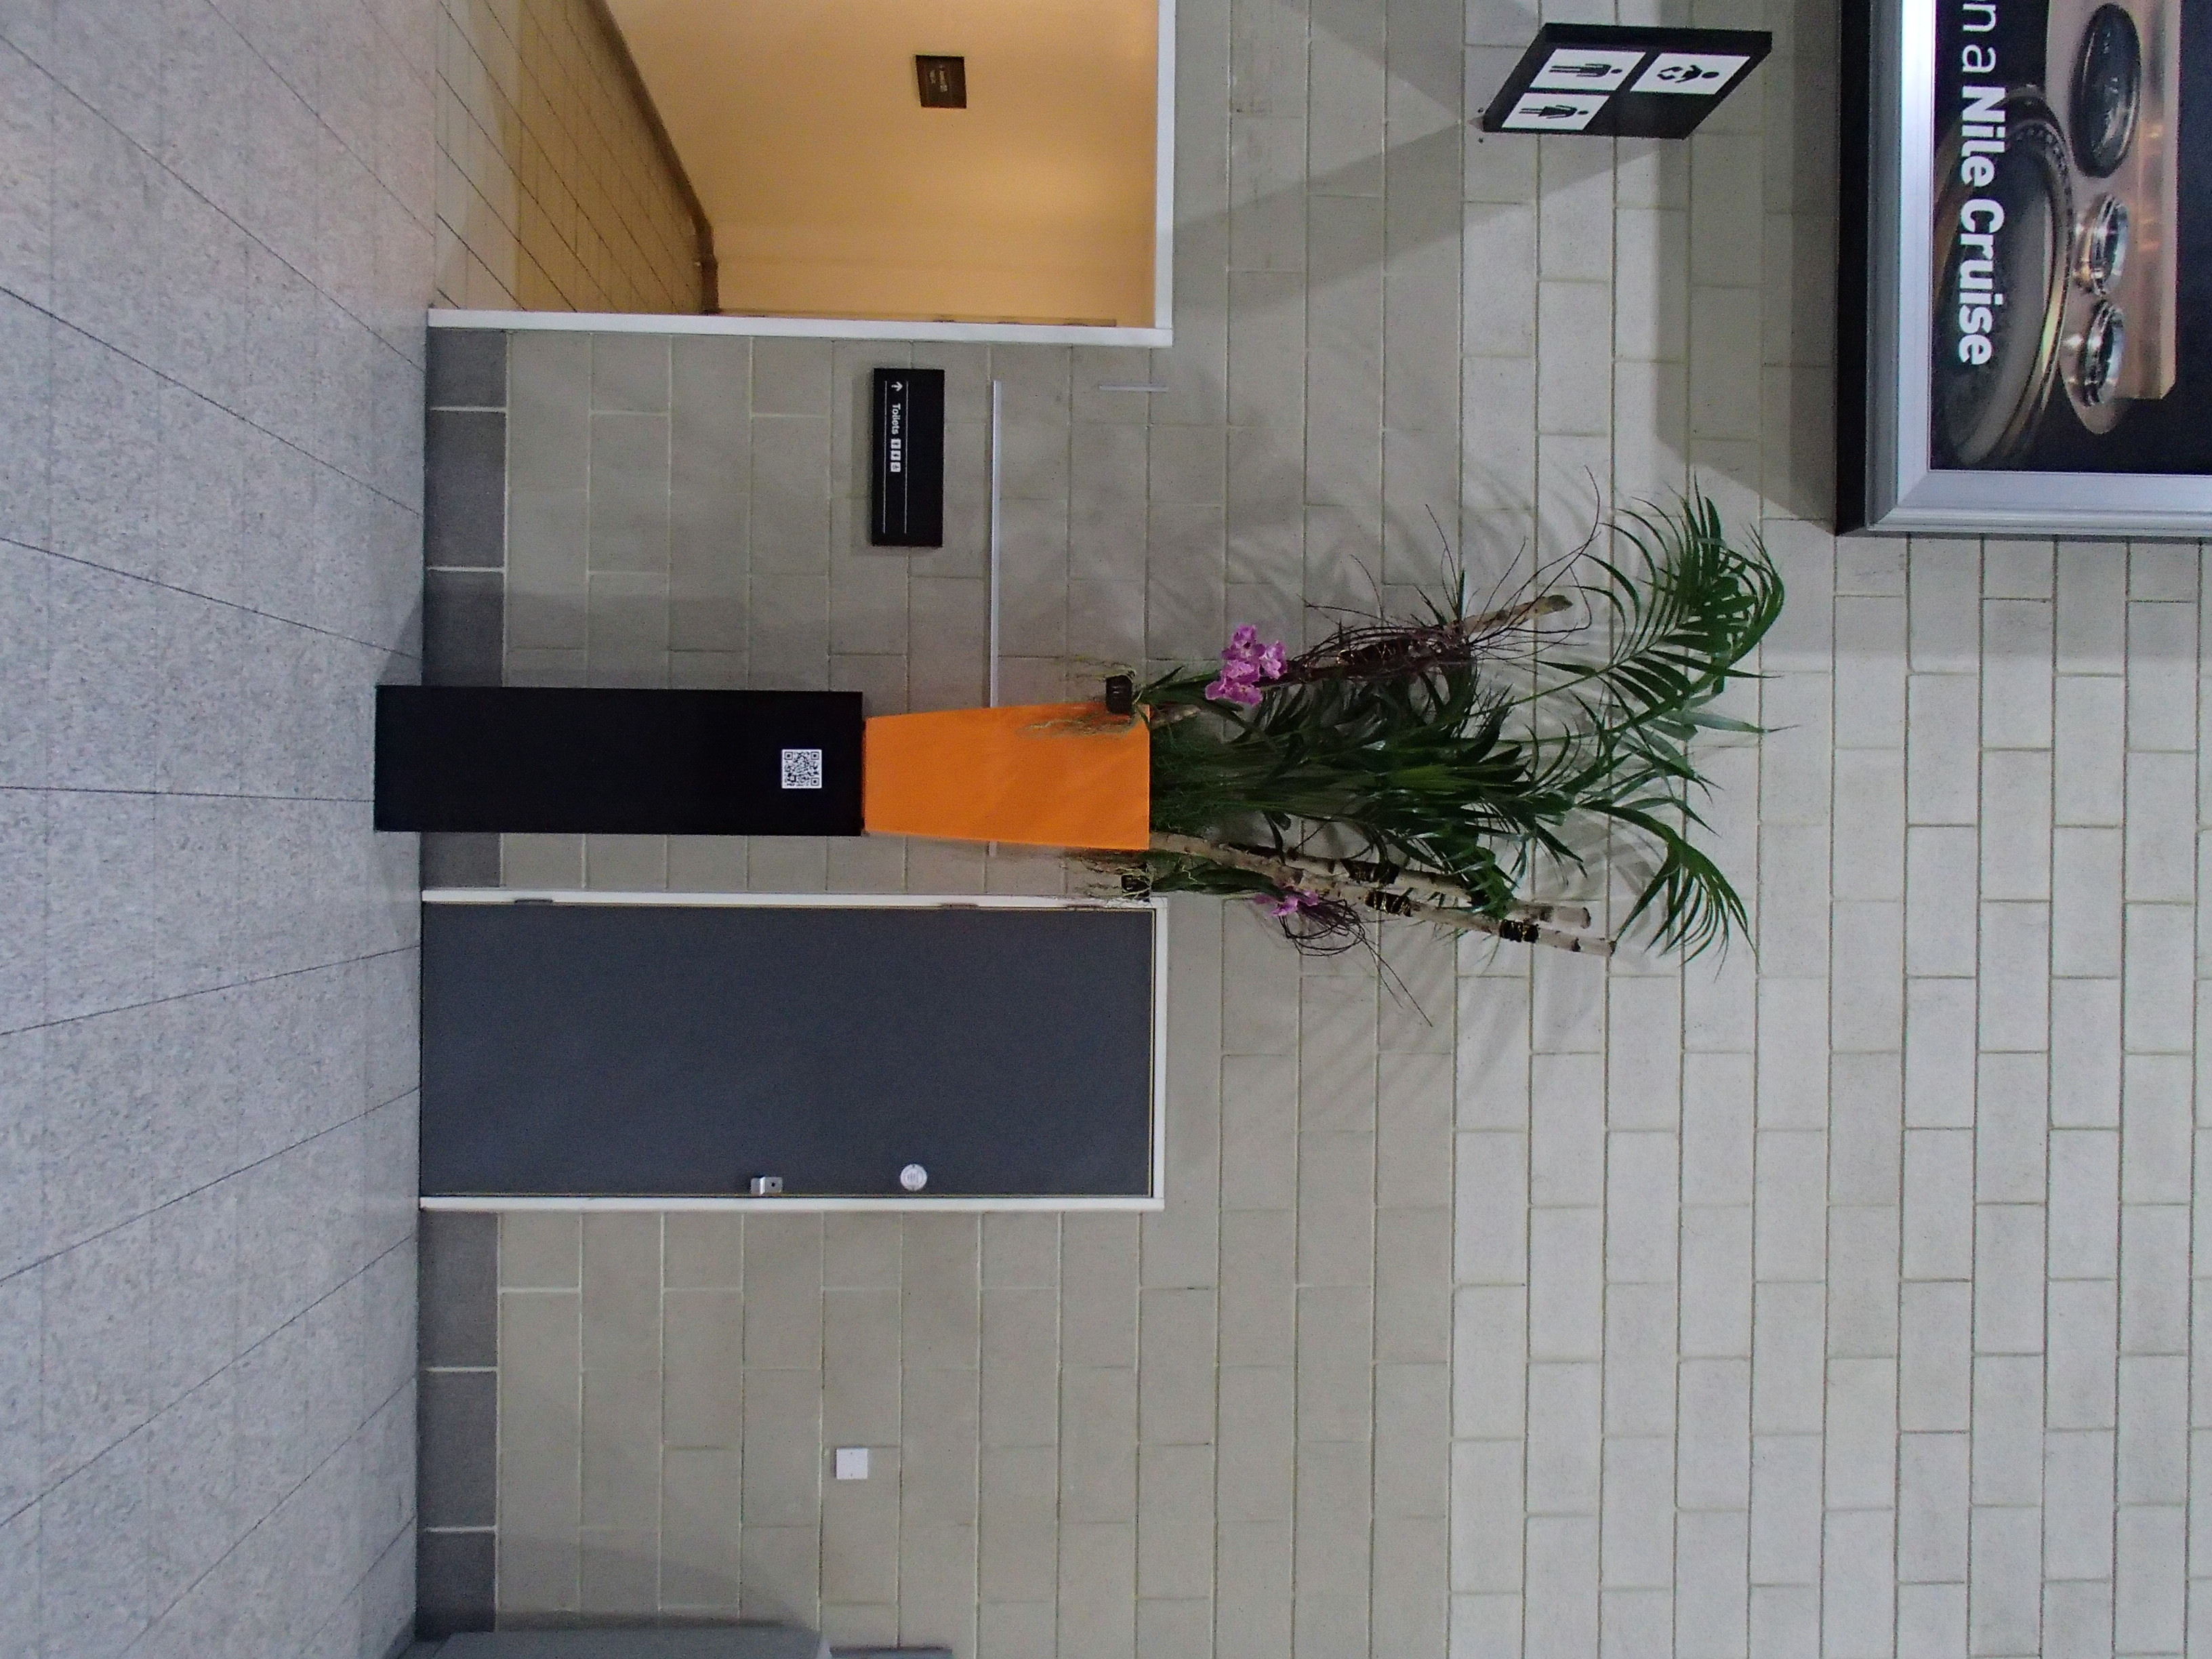
\includegraphics[width=\textwidth,angle=90]{figures/P1050143.JPG}
\caption{Plinth'd Nature}
\end{figure}

From a pedestal such as this one there is nothing further to be strived for but
full commune with the heavens. A small exemplar is chosen. Quickly, lightweight
channelling infrastructure is put in place, the thing is given an ``open top''.
Its delicate spread of antennae are placed out of arm's reach, the culturally
requisite lucky charms are added, disguised as decoration.

The base has wholly settled with the ground it sits on, happy to be so
possessed. This earthly protuberance that is relatively immovable plays host to
a splindly collection placed at the point where the thing gets as far as it
goes. From the simple guarantee of some weight something more contingent could
feel out (with imaginary hands) the safety to allow itself to emerge.

Simply put, this is technology manifest. A solid ``back box'' made of arcane
witchcraft lending stability to something otherwise intangible. Fragile human
emotion cradled gently by a larger process and so cradled allowed the space and
time to flourish generously to the delight of millions. There is almost a glow
about the thing, almost the sparkles of magic falling from its appendages. It
is how we know all is right with the world, we are in good company.

In this composition the perfect balance is struck in a sweep of asymmetry. An
image sails ahead unhanded and without guidance, forging a path of light and
leaving a spreading wake of shadows behind it. Standing in front of this
arrangement, this image of duality, the observer is thrown into a terrible and
relentless motion of their own. The coloured forms of the world shutter past at
pace, a cooling jet of histories and or of new ideas splashes on the brow and
spills away in dual rivers that meet between the shoulderblades. This is motion
without destination, as with ilynx and vertigo.

We see the expected, more human-scaled, more understandable artifacts of an
industrial construction; the visual clues that the thing as a whole did not
simply spring into existence, but rather came into being as the result of
repeated, tangental activity. The evidence appears as the side-effect of a
serious process, not as a direct mark. It arrives due to the neccesity of
silencing the pleas for care and attendance from smaller details, and instead
lending favour to the needs of the larger work taking place.

We have an acute angle into another world, a tranch of matter is used as bait
for something much larger, something which looking from here is already vested
with some largesse and power. A brief and delicious salad snack to goad the
creeping and splintered advances of a richly different existence across to this
relatively poor one.

The structure here, this thing, should at any moment leap into brief, hideous,
frenetic action as the chanceless, raw power of the universe carves a bolt
across eons, through timeless permanence and permanence, just to be in touch
with an object that will be there \emph{one time only}. This thing is a ``one
shot'' fabrication designed to take a massive but fleeting single input.

There is nothing to see here close up, \emph{so we stand back}. Not one amongst
us wants to have his eyebrows singed by the power of the infinite.

\chapter{Nature in the 80s}

\begin{figure}
\centering
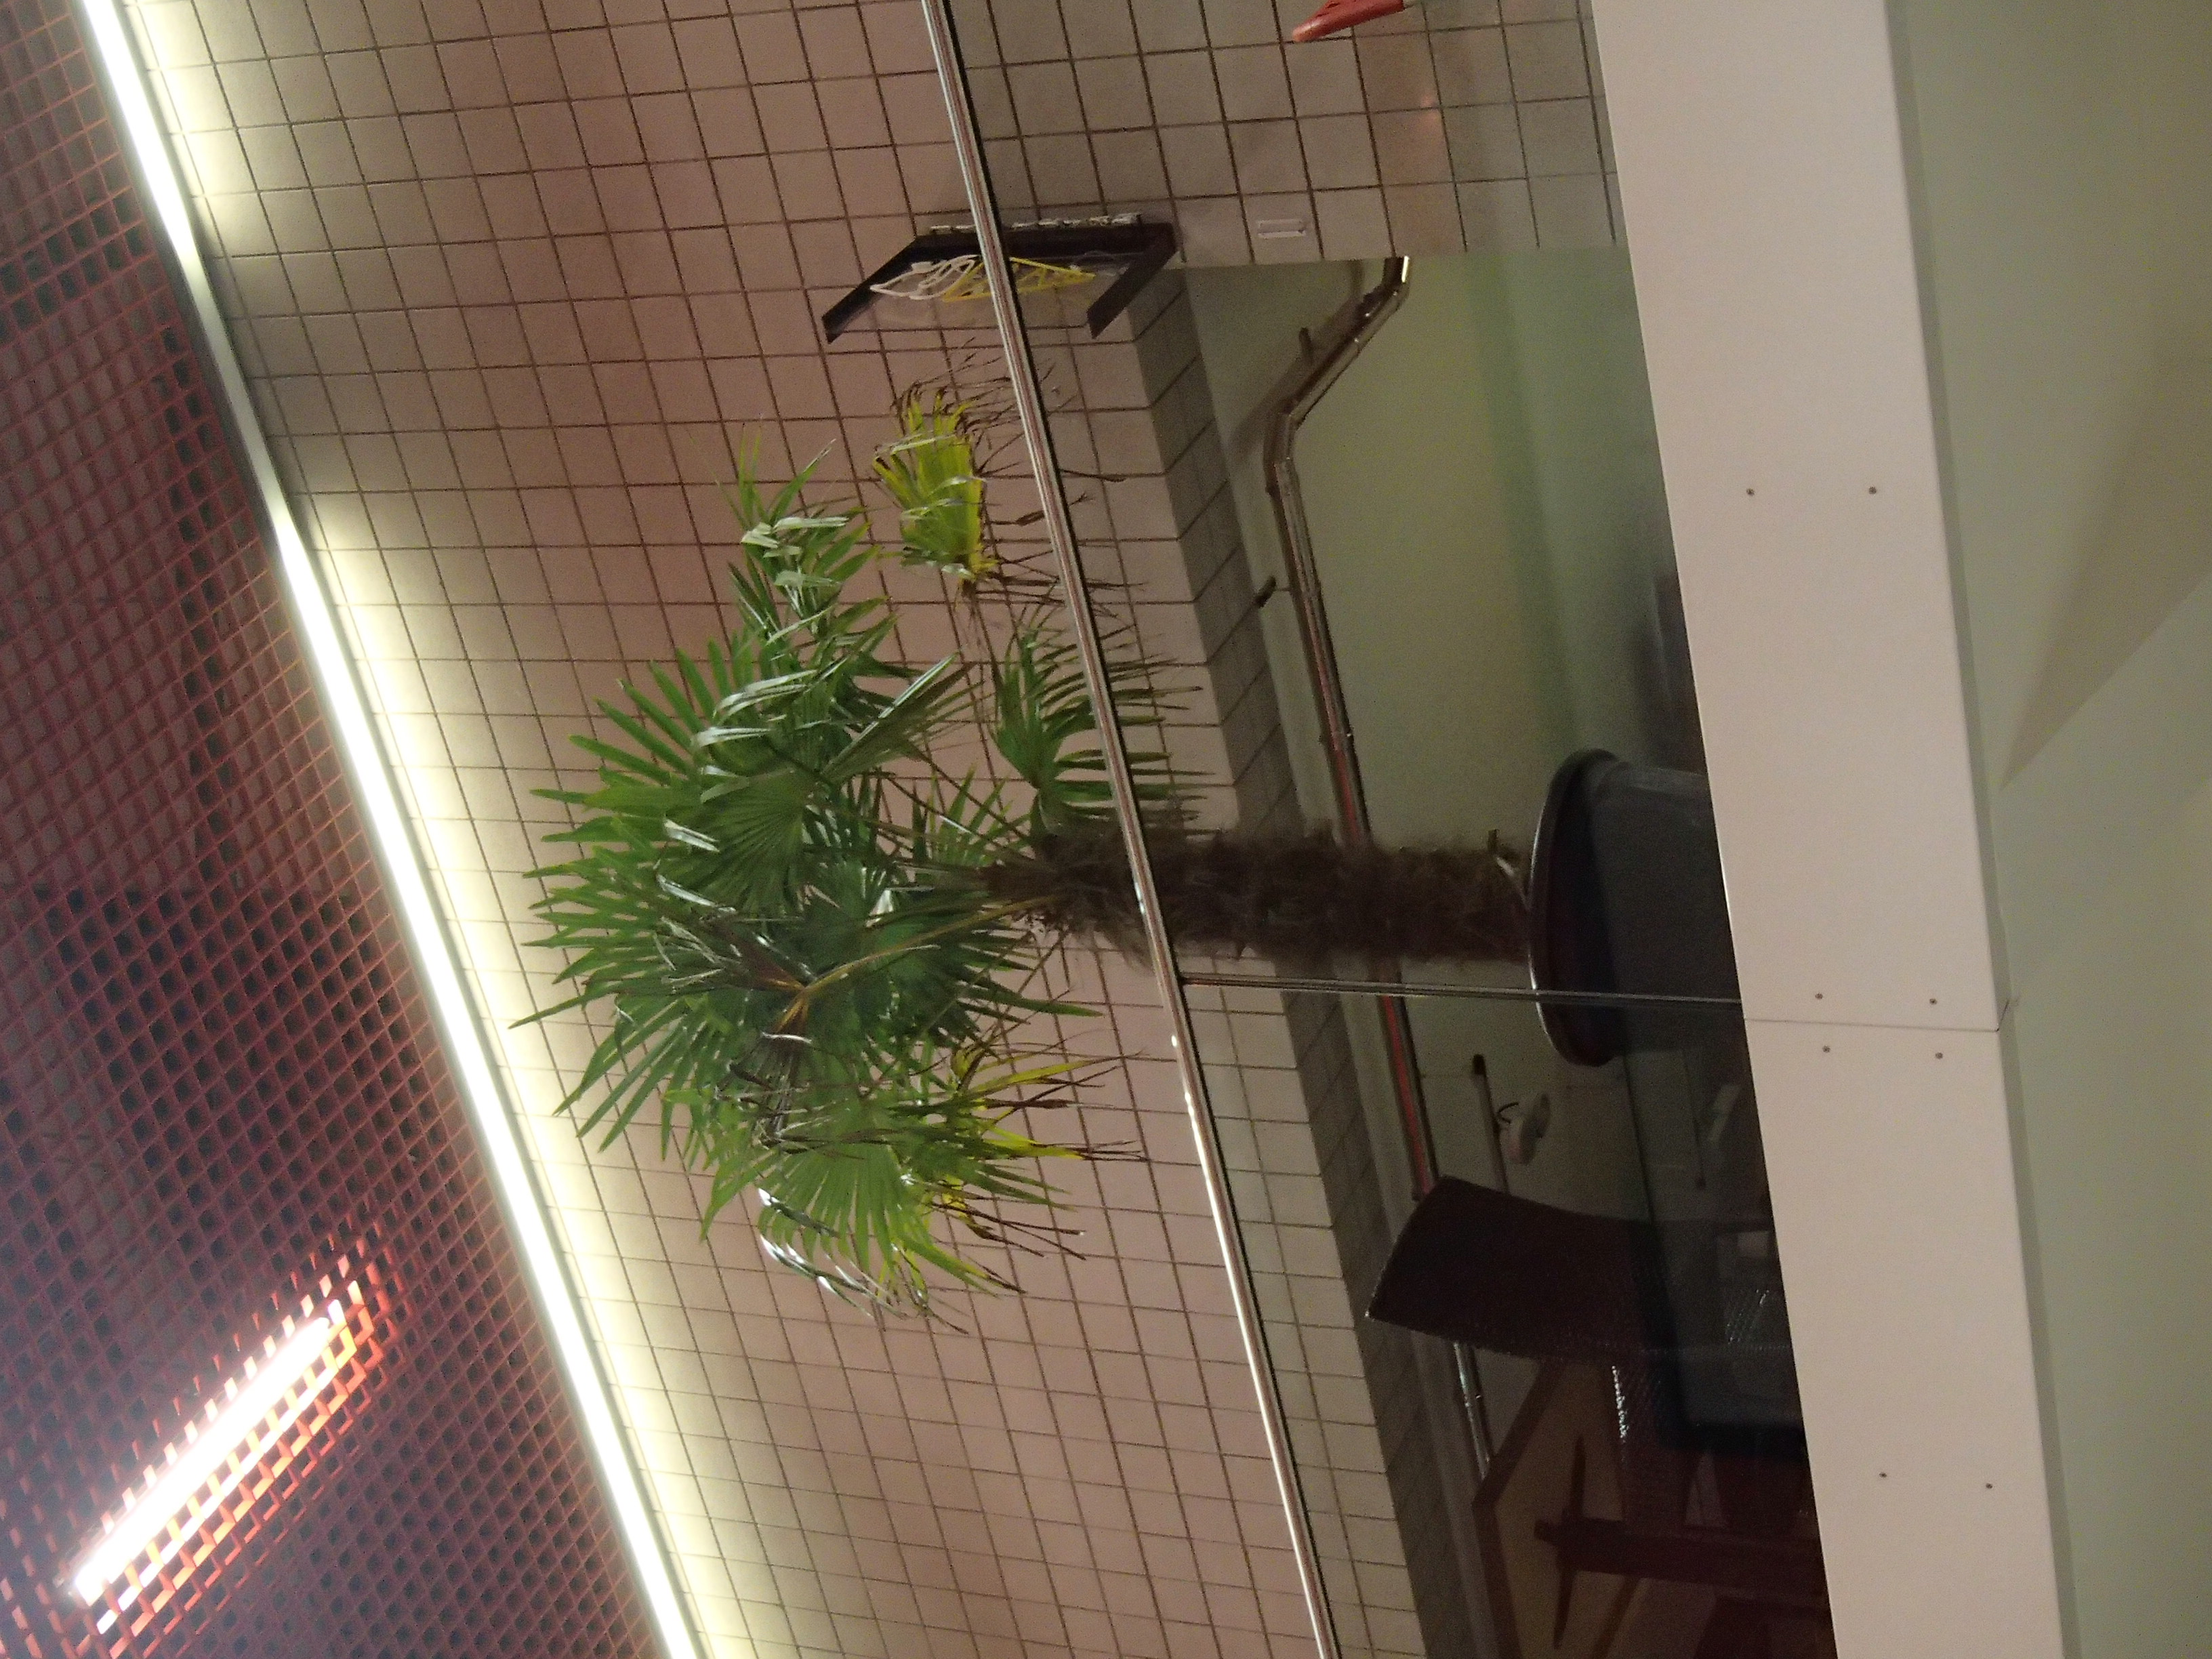
\includegraphics[width=\textwidth,angle=-90]{figures/P1050152.JPG}
\caption{Nature in the 80s}
\end{figure}

We don't remember what happened to us, just beginning to chase a new thought as
finance and oil exploded around us (in our midst). For a period nothing aged,
everything was \emph{as it was} and so it always would be. Our shared past, the
colloquial history of apes and animals was forgotten and cast aside in exchange
for this moment of shining clarity cast in shiny plastic.

At that time our human ``out-of-placeness'' became something commodifiable, the
hideous beast lurking within was invited (by advertising executives with wide
open arms and rather wild grins) to present itself pubicly in lavish media
form, fully out in the world. In this gesture the animal in man became a
caricature of itself, greeting and hollering. It was left outside, pathetically
soliciting for encouragement and accepting any given.

Even money as we knew it ceased to have proper meaning, instead finance became
a kind of de facto government. We would never again have the same need to fish
or farm or struggle we once did, there would be pure opportunity for every man
to \emph{have} the things he desired; living, as he was, in a bizarre new
democracy of home furnishings and rubberised kitchen utensils.

All things people could own became in some sense red, white and blue without
anyone intending them to be. Where before wealth had distinct and well-defined
characteristics, now a new formal aesthetic began to develop, eschewing
decoration and detail for ergonomics and ultilitarian elegance. The judgements
that for years could be made by studying the appearance of things suddenly
ceased to be hold water.  It became possible for validity to be built up and
broken down more quickly and in ways that were manageable by a greater
proportion of the populous. Civil society changed size over night.

The pure scale upon which society operated was parabolically altered; the shape
of things sagged.

To those with humanity's brightening prospects in mind, humanity's prospects
were considerably brightened. Social mobility looked promising and desirable,
the swelling of classed people was good fun, technology was just great and all
these things empowered people. However, it is often forgotten in politics that
pure power will not dilute, it only switches polarity at a greater rate. So as
winds changed, the peaceful lacuna formed by something like time delay or lag
time was rapidly and harshly emptied. Its inhabiants found themselves strewn
broadly across an unforgiving landscape.

They found nothing like home, their quiet was replaced by the hum of fridges
and the low thundering of traffic. The peace they found in image was exposed as
mere impoverished understanding; hypnosis by the flickering of a television
screen, without proper appreciation for the real messages transmitted there.

Some stayed mobile, some just stayed. Maudlin denizens of a place that had had
its promise turned to ash. Now surrounded by bars and grids but still living,
seeming to the outside world all but montionless, making the quiet statement
\emph{``you don't have me like that''} by grimly singing low the songs of the
old country.

Indeed, some music could pass and stayed with them, but was only permitted when
accompanied by proper documentation and even then only through appropriate
channels.

The world became too big and too empty and too flat, but these ex-regal figures
remained raised. They stood for weak beacons to their counterparts, thinly
sounding out a kind of stiff moisture against the overprescent smell of ozone.
In a scene of collapsing dust and the dry stains of ventilation they were the
small, shabby originals impossibly returning to their overblown simulacra.

We had no choice but to see them welcomed ``in'', there was too much sharing of
evolutionary roots; formal structure, growth patterns, etc. But, despite the
commonality, they existed differently in time. One was nourished by its passing
and the other was slowly beaten back by it. These individual relationships
essentially hid each from the other by an unassailable chasm of scale.

\chapter{Cornered Nature No. 1}

\begin{figure}
\centering
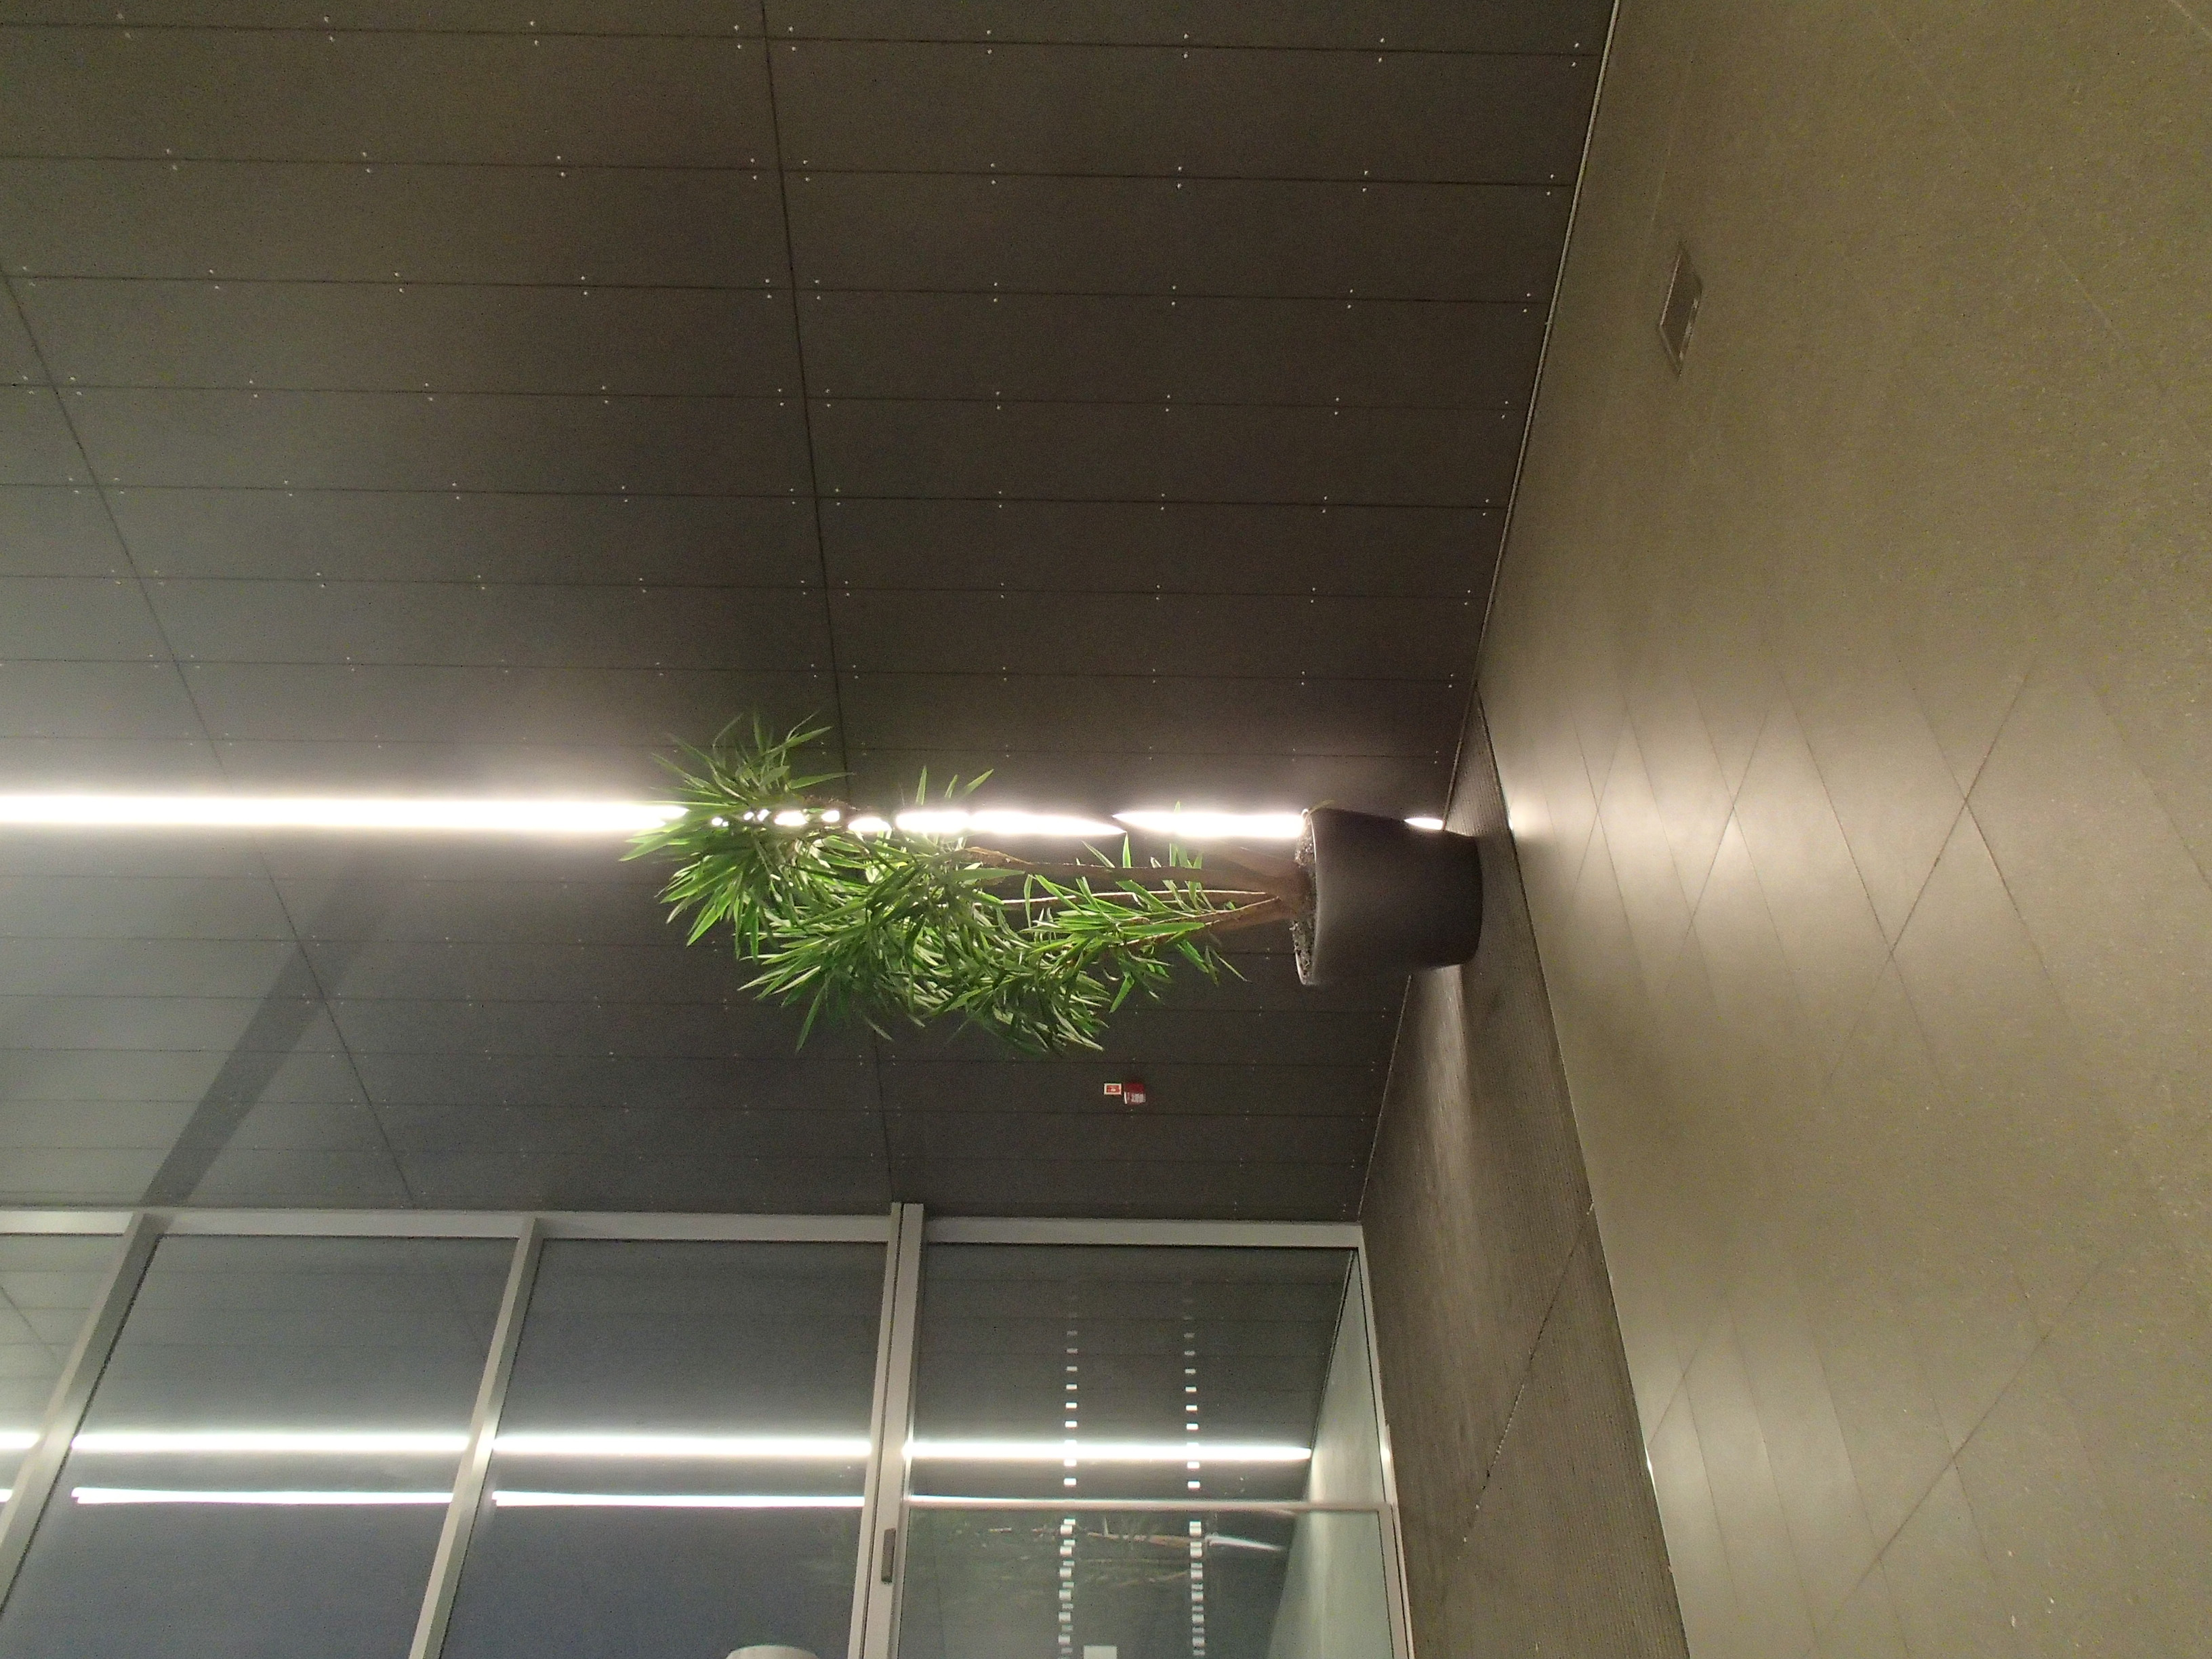
\includegraphics[width=\textwidth,angle=-90]{figures/P1050156.JPG}
\caption{Cornered Nature No. 1}
\end{figure}

Like most all defensive pretended misunderstanding, a body acting as if it
doesn't have any regard for its proper form is to be viewed as tragicomic.

\chapter{Cornered Nature No. 2}

\begin{figure}
\centering
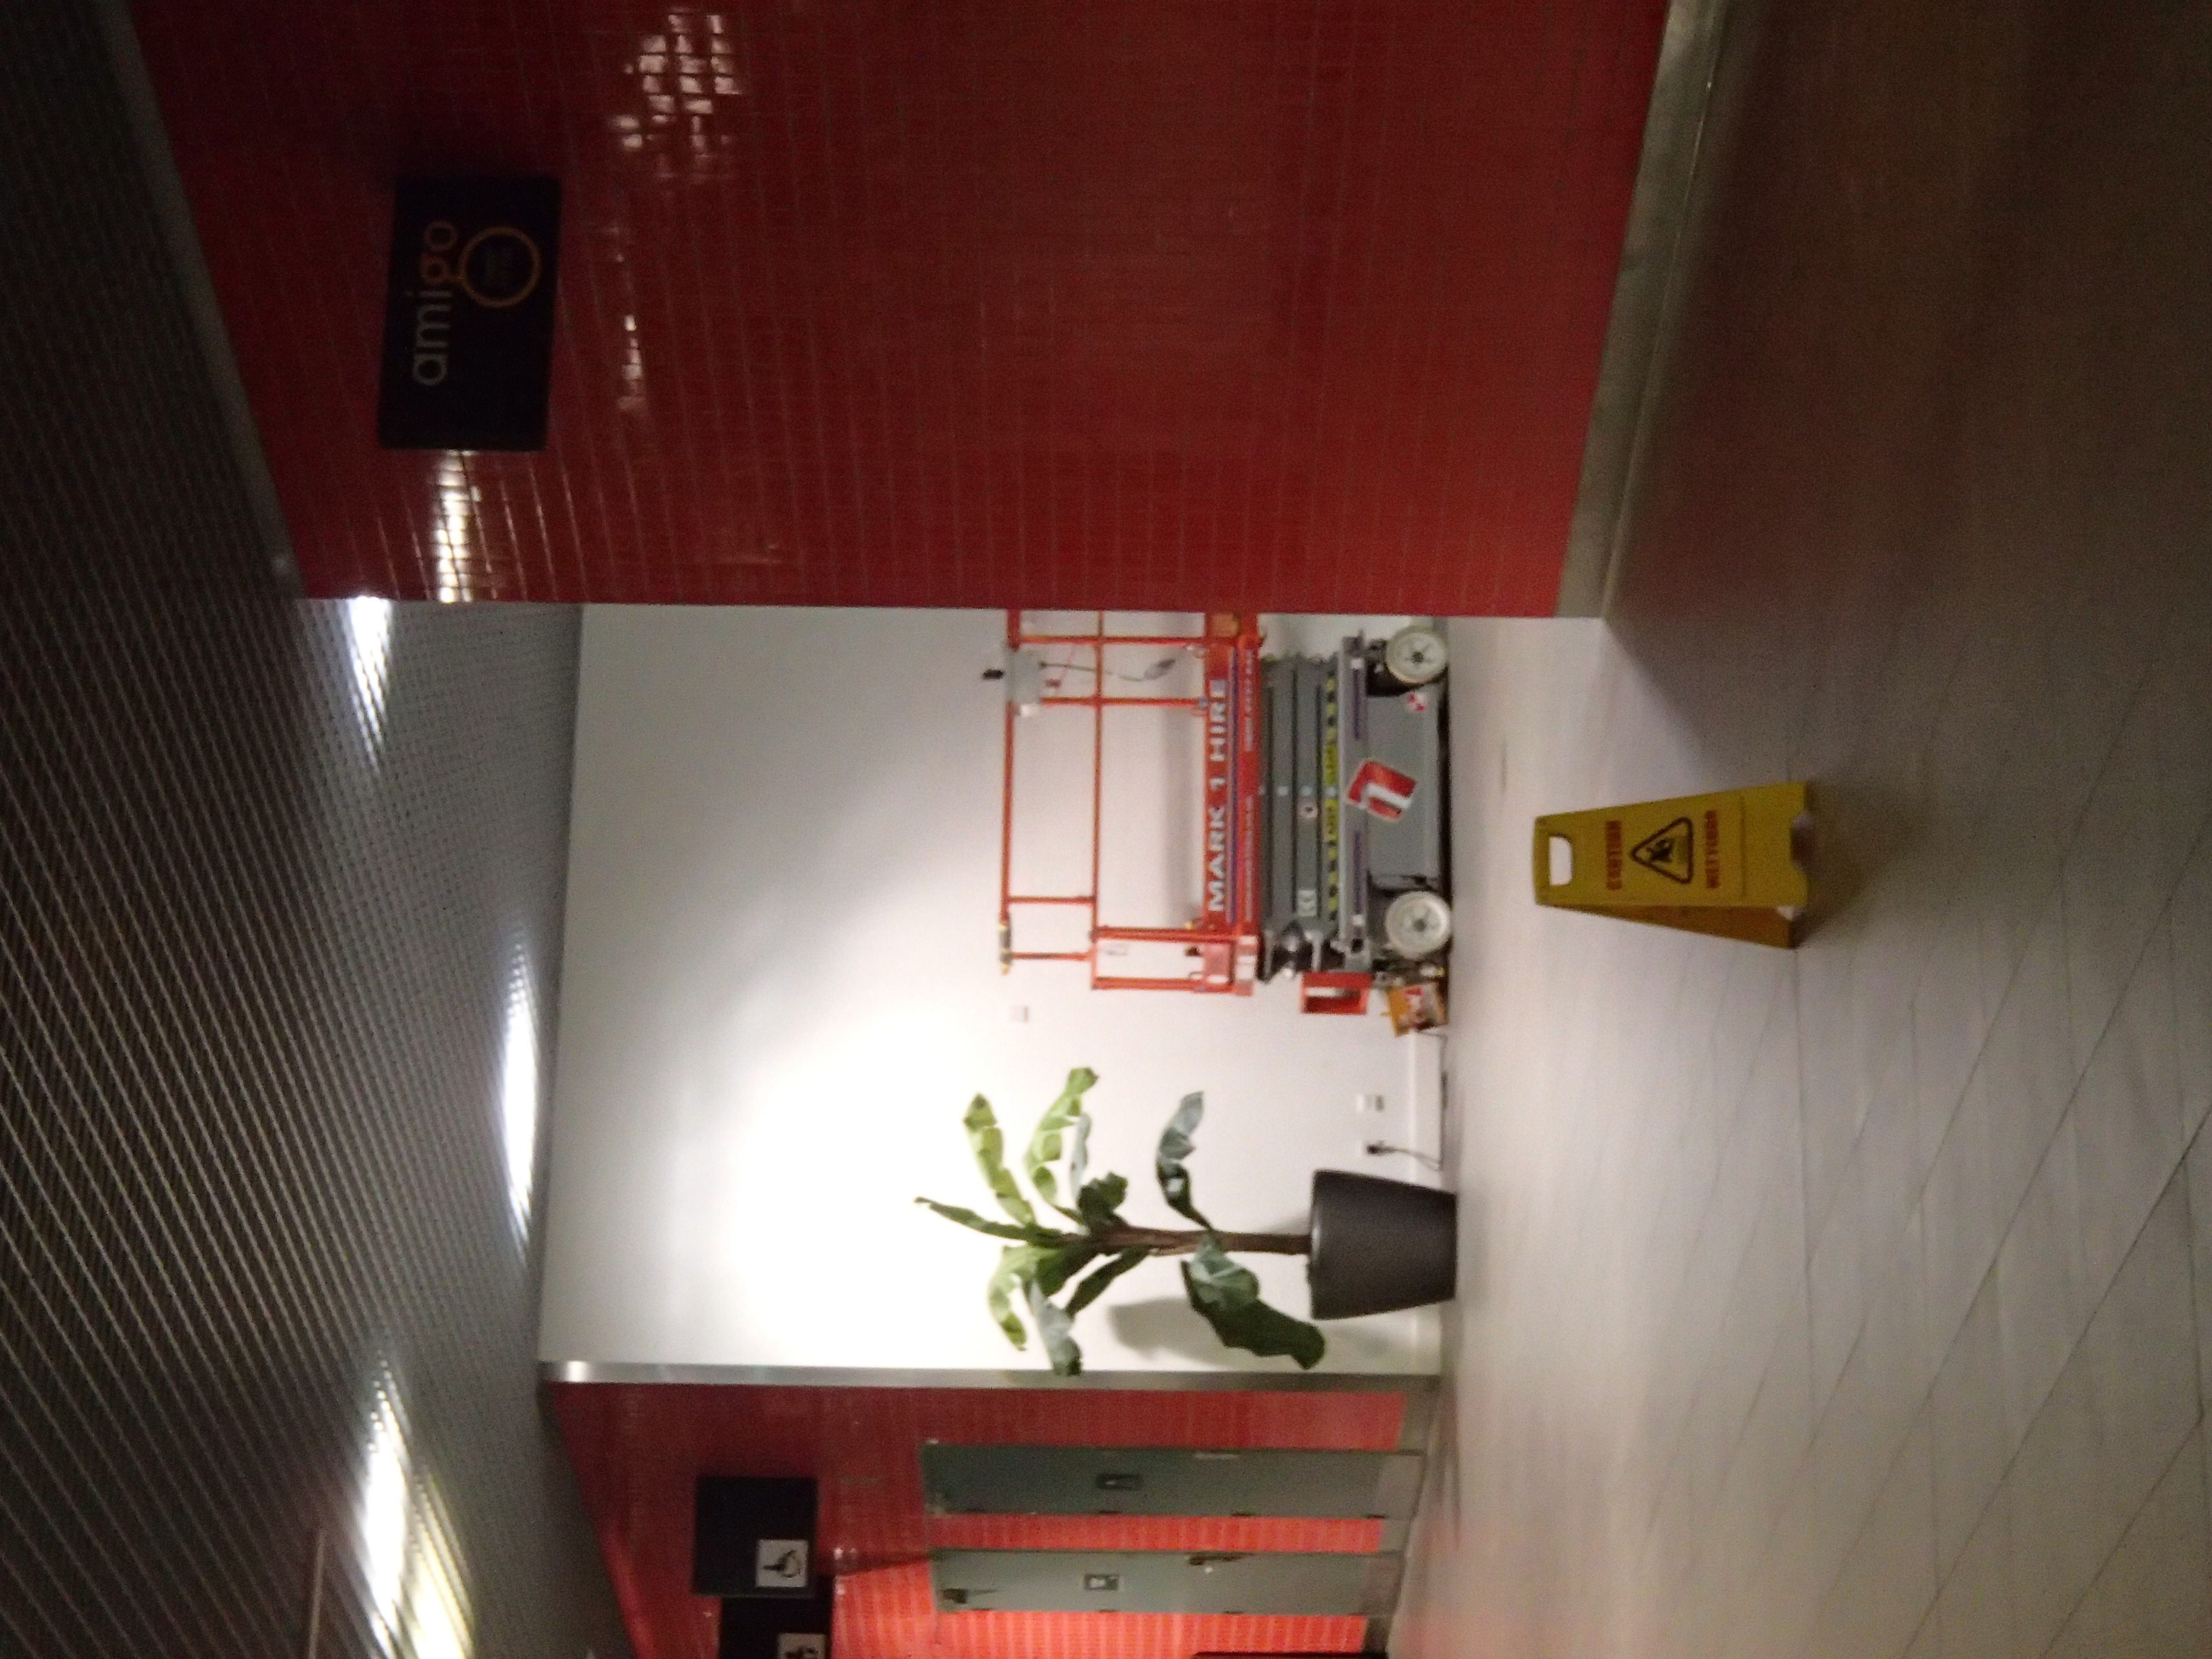
\includegraphics[width=\textwidth,angle=-90]{figures/P1050158.JPG}
\caption{Cornered Nature No. 2}
\end{figure}

\chapter{Nature Addendum}

\begin{figure}
\centering
\includegraphics[width=0.76\textwidth]{figures/20131116-1403-04.jpg}
\caption{Nature Addendum}
\end{figure}

\end{document}
